\chapter{Unfolding studies}

\label{ch:appendix_unfoldingStudies}

\vspace{-35pt}
\begin{figure}[hb] 
    \centering
    {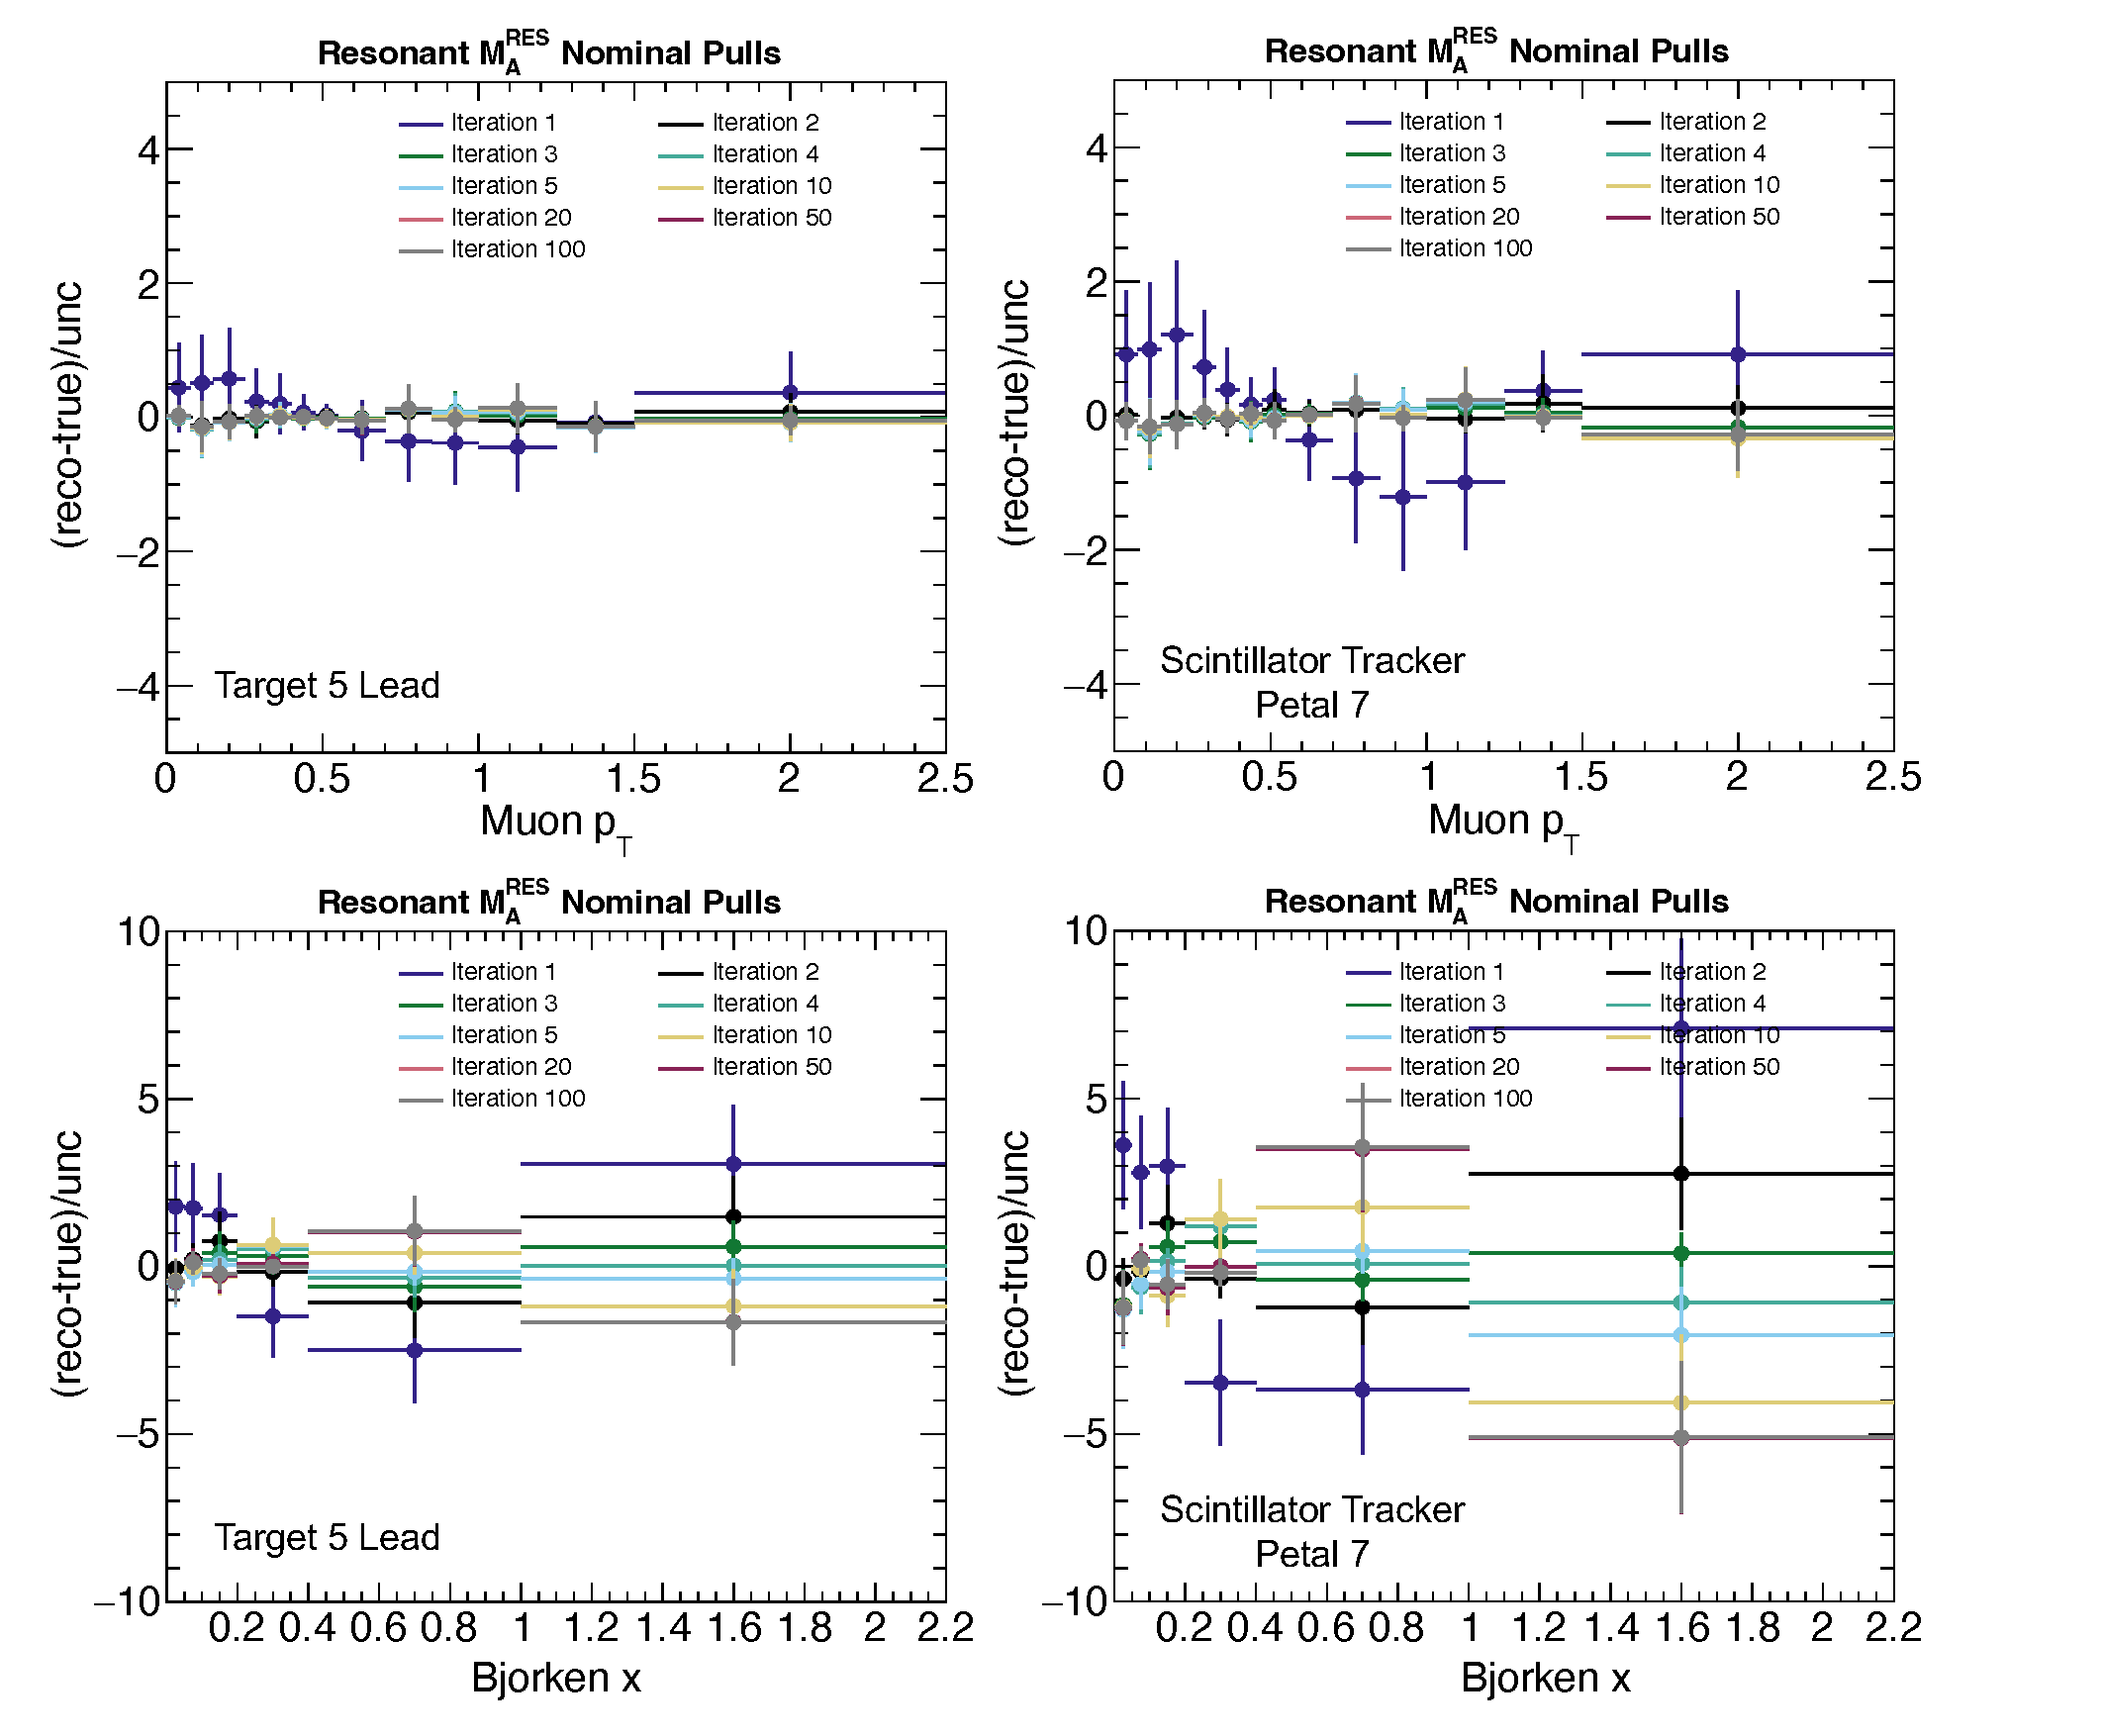
\includegraphics[width=0.95\textwidth]{07analysis1D/figures/maresWarp_lead5tracker7_pTx_pulls.pdf}}%
    \caption{Pull distributions for the 'Resonant $M_{A}^{\text{RES}}$ nominal' warping study are presented for target 5 lead (left panel) and the scintillator tracker petal 7 (right panel) in both antimuon $p_{\text{T}}$ (top) and Bjorken $x$ (bottom). In the case of $p_{\text{T}}$, both pull distributions illustrate a reduction in bias with each iteration of the unfolding process. However, for the Bjorken $x$ pull distribution, especially at high Bjorken $x$, there is an indication of some divergence, which prompted further investigation into potential model dependence.}
    %[short caption] {long caption}
    \label{fig:warpingMaRes_pulls}
\end{figure}

\begin{figure}[b!] 
    \centering
    {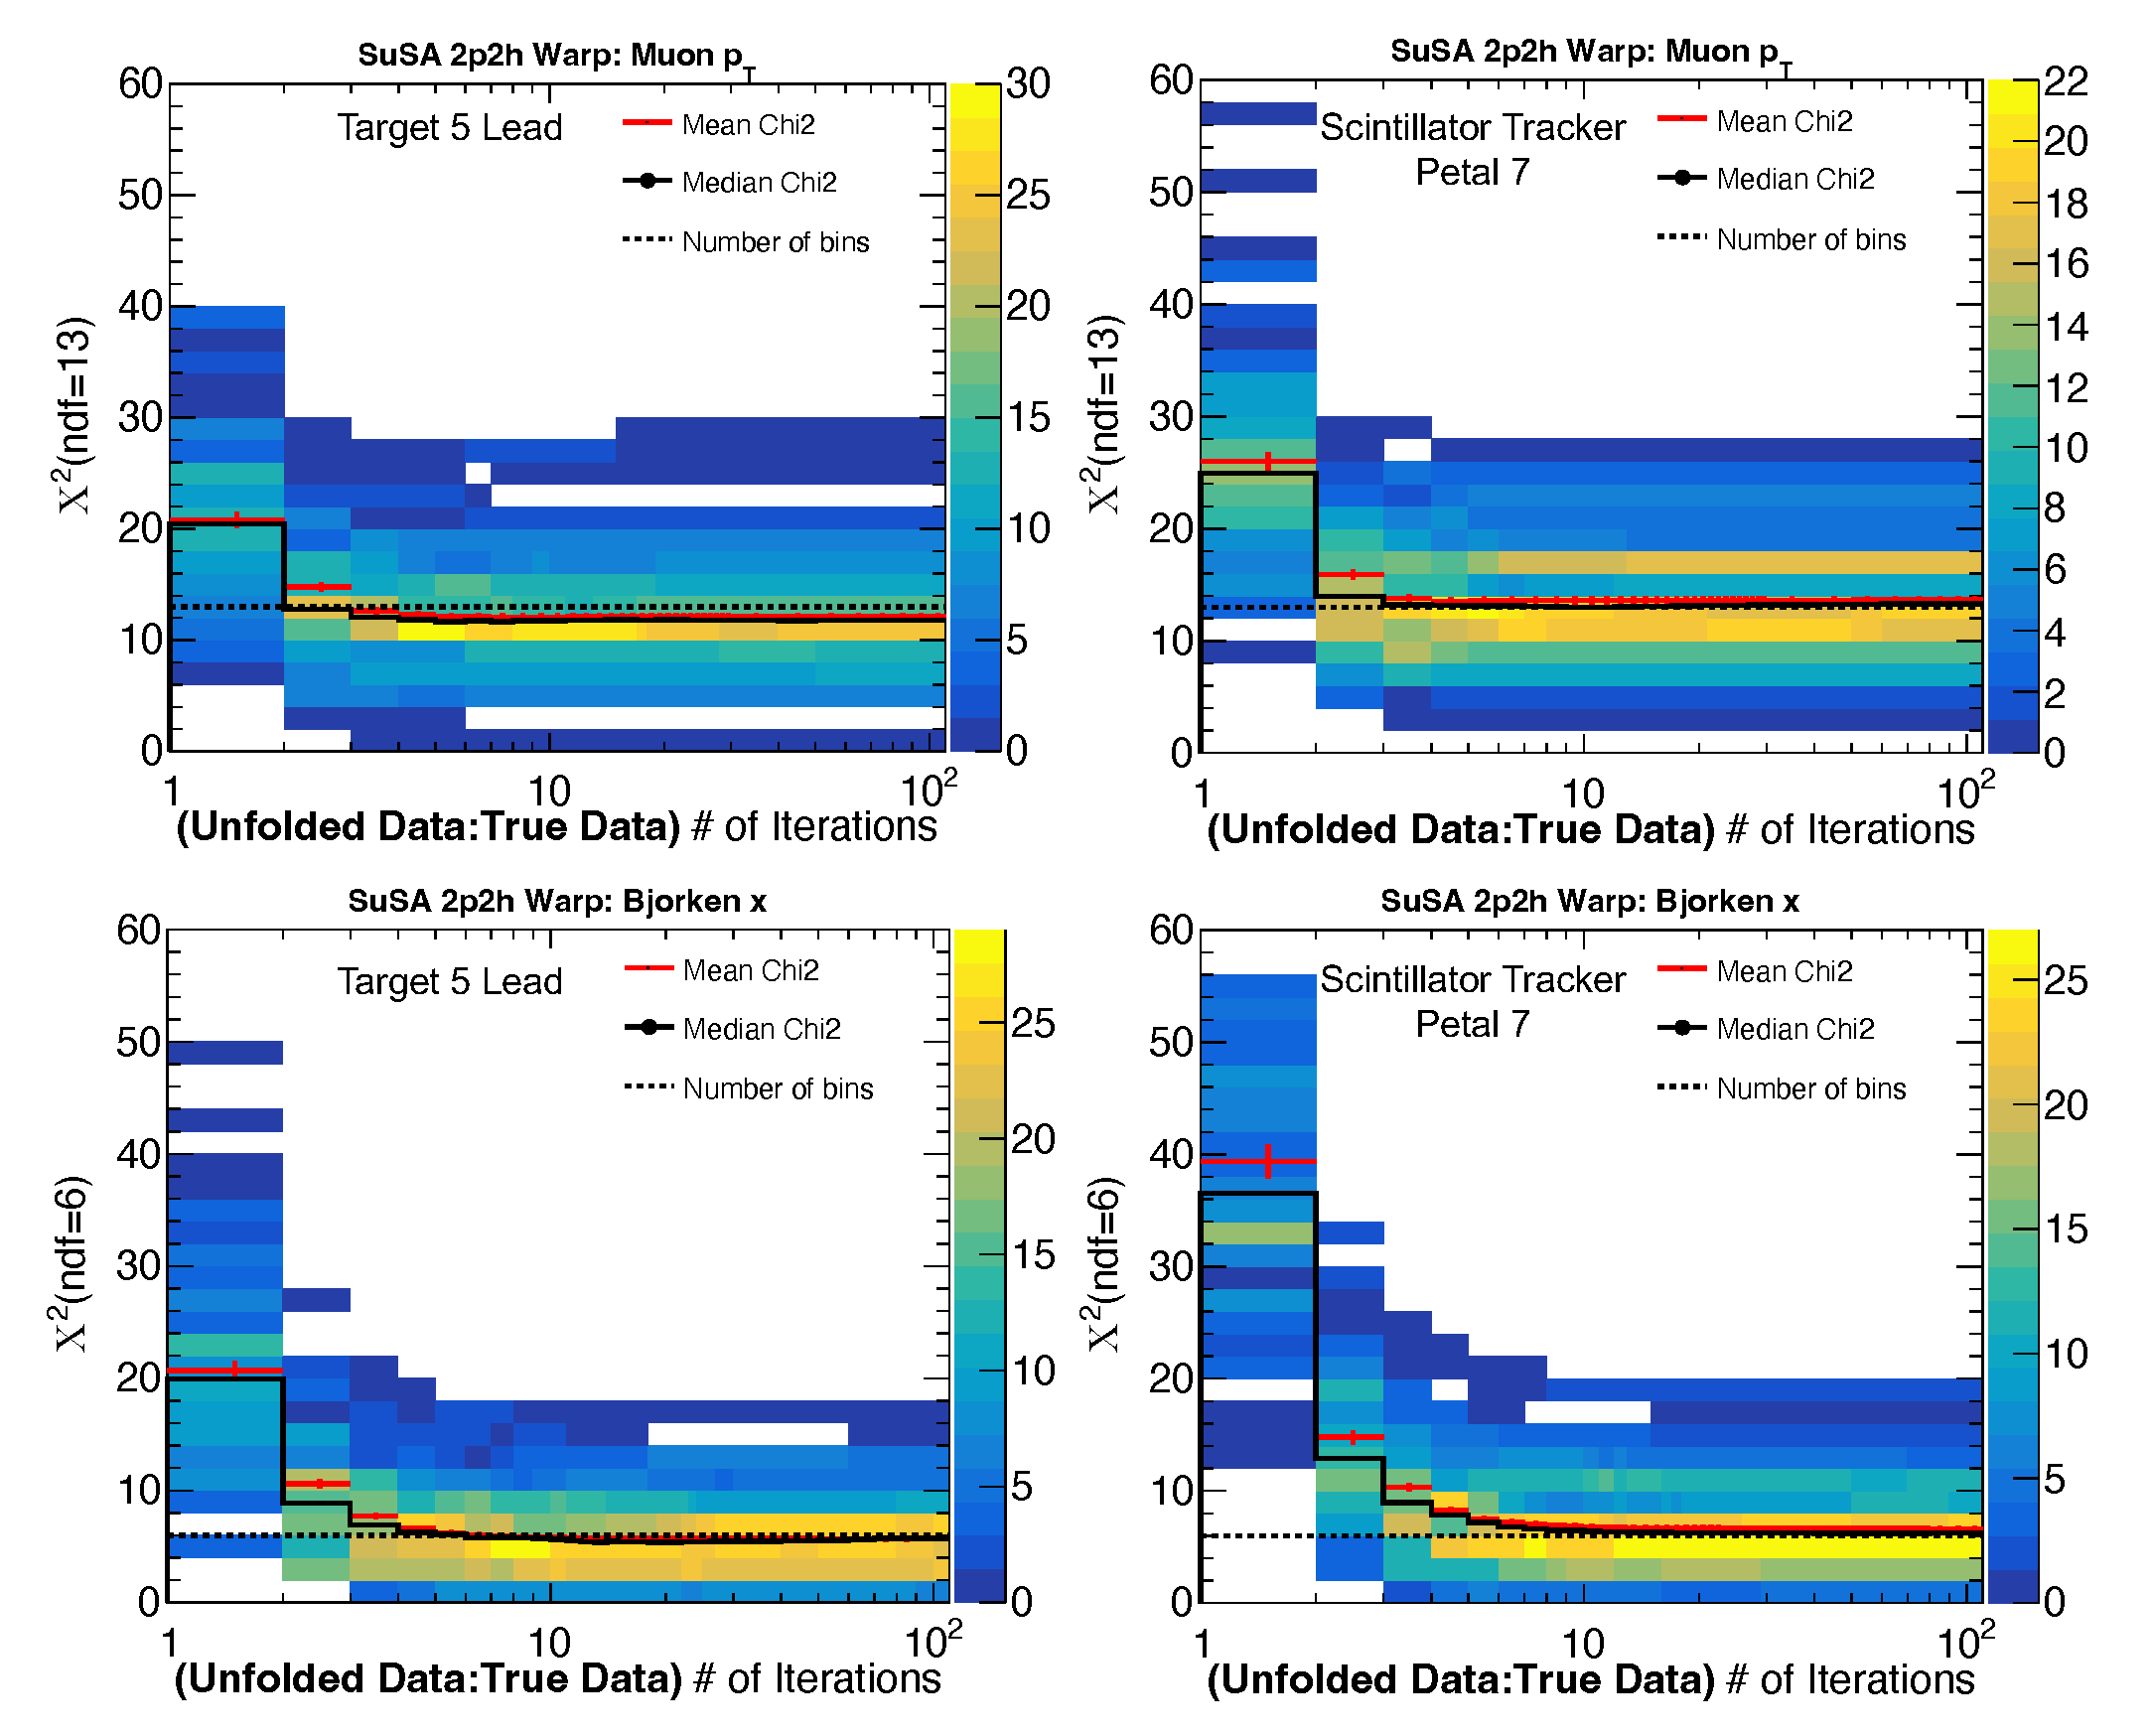
\includegraphics[width=1\textwidth]{07analysis1D/figures/susaWarp_lead5tracker7_pTx.pdf}}%
    \caption{The 'SuSA 2p2h' warping study conducted for target 5 lead (left panel) and the scintillator tracker petal 7 (right panel) in both antimuon $p_{\text{T}}$ (top) and Bjorken $x$ (bottom). Each heatmap displays the calculated $\chi^2$ between the unfolded and true distribution of the warped model as a function of the number of iterations for each of the 100 Poisson throws. The solid lines represent the median and mean $\chi^2$, while the dashed line indicates the number of bins or degrees of freedom (ndf). Both in $p_{\text{T}}$ and Bjorken $x$, the median $\chi^2$ stabilises at the ndf after several iterations indicating minimal bias.}
    %[short caption] {long caption}
    \label{fig:warpingSuSA}
\end{figure}

\begin{figure}%
    \vspace{-25pt}
    \centering
    \subfloat{{\includegraphics[width=0.5\textwidth]{thesisFigures/warpingStudies/MaRESwarp_xsec_check/crossSection_Daisy_t3_z06_x_minervame5A6A6B6C6D6E6F6G6H6I6J_DifferentCVComparison_Data.pdf} }}%
    \qquad
    \hspace{-40pt}
    \subfloat{{\includegraphics[width=0.5\textwidth]{thesisFigures/warpingStudies/MaRESwarp_xsec_check/crossSection_Daisy_t235_z26_x_minervame5A6A6B6C6D6E6F6G6H6I6J_DifferentCVComparison_Data.pdf} }}%
    \qquad
    \subfloat{{\includegraphics[width=0.5\textwidth]{thesisFigures/warpingStudies/MaRESwarp_xsec_check/crossSection_Daisy_t2345_z82_x_minervame5A6A6B6C6D6E6F6G6H6I6J_DifferentCVComparison_Data.pdf} }}%
    \qquad
    \hspace{-40pt}
    \subfloat{{\includegraphics[width=0.5\textwidth]{thesisFigures/warpingStudies/MaRESwarp_xsec_check/crossSection_t99_z99_x_minervame5A6A6B6C6D6E6F6G6H6I6J_DiffrentCVComparison_Data.pdf} }}%
    \caption{Comparison of the data cross-section for carbon (top left), iron (top right), lead (bottom left) and scintillator (bottom right) as a function of Bjorken $x$ extracted with the original simulation and `Resonant $M_{A}^{\text{RES}}$ nominal' central value to investigate potential model dependence.}
    %\vspace{0pt}}%
    \centering
    \subfloat{{\includegraphics[width=0.5\textwidth]{thesisFigures/warpingStudies/MaRESwarp_xsec_check/xSec_ratio_Daisy_t3_z06_x_minervame5A6A6B6C6D6E6F6G6H6I6J_DifferentCVComparison_Data.png} }}%
    \qquad
    \hspace{-40pt}
    \subfloat{{\includegraphics[width=0.5\textwidth]{thesisFigures/warpingStudies/MaRESwarp_xsec_check/xSec_ratio_Daisy_t235_z26_x_minervame5A6A6B6C6D6E6F6G6H6I6J_DifferentCVComparison_Data.pdf} }}%
    \caption{Comparison of the carbon-to-scintillator (left) and iron-to-scintillator (right) data cross-section ratio as a function of Bjorken $x$ extracted with the original simulation and `Resonant $M_{A}^{\text{RES}}$ nominal' central value. The central values of the data cross-section extracted using the warped model are encompassed by the total uncertainty (including the systematic, represented by the outer error bars) of the data cross-section extracted using the original simulation. This indicates that any potential model dependence is covered by the underlying uncertainty.}%
\end{figure}

\begin{figure}%
    \centering
    \subfloat{{\includegraphics[width=0.5\textwidth]{thesisFigures/warpingStudies/invisibleEnergyVariation/crossSection_Daisy_t3_z06_x_minervame5A6A6B6C6D6E6F6G6H6I6J_InvisibleEnergyVariation_Data.pdf} }}%
    \qquad
    \hspace{-40pt}
    \subfloat{{\includegraphics[width=0.5\textwidth]{thesisFigures/warpingStudies/invisibleEnergyVariation/crossSection_Daisy_t235_z26_x_minervame5A6A6B6C6D6E6F6G6H6I6J_InvisibleEnergyVariation_Data.pdf} }}%
    \qquad
    \subfloat{{\includegraphics[width=0.5\textwidth]{thesisFigures/warpingStudies/invisibleEnergyVariation/crossSection_Daisy_t2345_z82_x_minervame5A6A6B6C6D6E6F6G6H6I6J_InvisibleEnergyVariation_Data.pdf} }}%
    \qquad
    \hspace{-40pt}
    \subfloat{{\includegraphics[width=0.5\textwidth]{thesisFigures/warpingStudies/invisibleEnergyVariation/crossSection_t99_z99_x_minervame5A6A6B6C6D6E6F6G6H6I6J_InvisibleEnergyVariation_Data.pdf} }}%
    \caption{Comparison of the data cross-section for carbon (top left), iron (top right), lead (bottom left) and scintillator (bottom right) as a function of Bjorken $x$ extracted with the original simulation and `Invisible energy 10\%' central value to investigate model dependence arising from neutron modelling.}%
    \centering
    \subfloat{{\includegraphics[width=0.5\textwidth]{thesisFigures/warpingStudies/invisibleEnergyVariation/xSec_ratio_Daisy_t3_z06_x_minervame5A6A6B6C6D6E6F6G6H6I6J_InvisibleEnergyVariation_Data.pdf} }}%
    \qquad
    \hspace{-40pt}
    \subfloat{{\includegraphics[width=0.5\textwidth]{thesisFigures/warpingStudies/invisibleEnergyVariation/xSec_ratio_Daisy_t235_z26_x_minervame5A6A6B6C6D6E6F6G6H6I6J_InvisibleEnergyVariation_Data.pdf} }}%
    \caption{Comparison of the carbon-to-scintillator (left) and iron-to-scintillator (right) data cross-section ratio as a function of Bjorken $x$ extracted with the original simulation and `Invisible energy 10\%' central value to investigate model dependence arising from neutron modelling, revealing possible bias in the $x > 1$ bin.}%
\end{figure}
\vspace{-50pt}
\begin{figure}%
    \centering
    \subfloat{{\includegraphics[width=0.5\textwidth]{thesisFigures/warpingStudies/additionalStatUnc/Warping_t5_z82_minervame5A6A6B6C6D6E6F6G6H6I6J_cv_x_fStudy.pdf} }}%
    \qquad
    \hspace{-40pt}
    \subfloat{{\includegraphics[width=0.5\textwidth]{thesisFigures/warpingStudies/additionalStatUnc/Warping_t99_z99_minervame5A6A6B6C6D6E6F6G6H6I6J_cv_x_7_fStudy.pdf} }}%
    \caption{Correction factor $F$ to the statistical uncertainty of the unfolded sample due to finite size of the simulation in the migration matrix for target 5 lead and the scintillator tracker petal 7 in Bjorken $x$. The solid lines illustrate that at the selected number of iterations, i.e. 9 iterations, the calculated $\chi^2$ between the unfolded and true simulation converges to the number of degrees of freedom (dashed line) for the $F$ factor 4 and 4.5 for target 5 lead and the scintillator tracker petal 7 respectively.}%
\end{figure}

